\scanpage{60}
-VII- 19 - \hfill n° 383

\uline{Système de racines de type} $G_2$

\figure{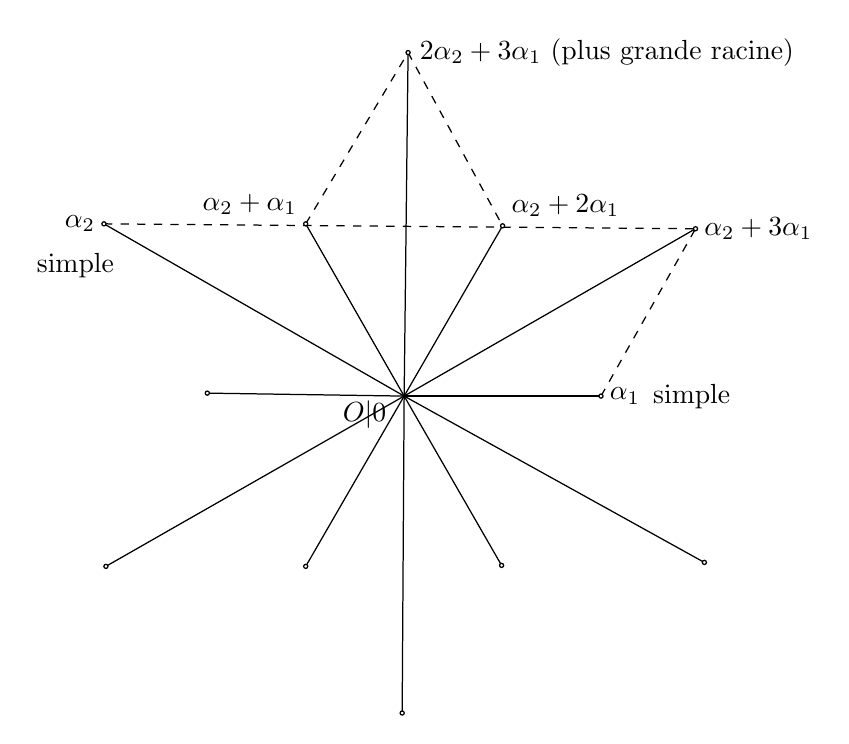
\begin{tikzpicture}[x=1.25cm,y=1.25cm,line width=.45pt]
\coordinate (O) at (0,0);
\coordinate (a) at (2,0);
\coordinate (b) at (-3.05,1.75);
\coordinate (c) at (-1,1.75);
\coordinate (d) at (1,1.73);
\coordinate (e) at (2.96,1.70);
\coordinate (f) at (.04,3.49);
\coordinate (na) at (-2,.03);
\coordinate (nb) at (3.05,-1.69);
\coordinate (nc) at (.99,-1.72);
\coordinate (nd) at (-1,-1.73);
\coordinate (ne) at (-3.03,-1.73);
\coordinate (nf) at (-.02,-3.22);
\draw[dashed] (b)--(e);
\draw[dashed] (c)--(f)--(d);
\draw[dashed] (a)--(e);
\foreach \p in {a,b,c,d,e,f,na,nb,nc,nd,ne,nf}{\draw (O)--(\p);\draw[fill=white] (\p) circle (.021);}
\node[below left,inner sep=2pt] at (-.12,.02) {$\unsure{O|0}$};
\node[right,inner sep=3pt] at (a) {$\alpha_1$};
\node[right] at (2.43,0) {simple};
\node[left,inner sep=3pt] at (b) {$\alpha_2$};
\node[below] at (-3.34,1.55) {simple};
\node[above left,inner sep=3pt] at (c) {$\alpha_2+\alpha_1$};
\node[above right,inner sep=3pt] at (d) {$\alpha_2+2\alpha_1$};
\node[right,inner sep=3pt] at (e) {$\alpha_2+3\alpha_1$};
\node[right,inner sep=4pt] at (f) {$2\alpha_2+3\alpha_1$ (plus grande racine)};
\end{tikzpicture}}
\mspage{59}
